\documentclass[10pt,twocolumn,letterpaper]{article}

\usepackage{cvpr}
\usepackage{times}
\usepackage{epsfig}
\usepackage{graphicx}
\usepackage{amsmath}
\usepackage{amssymb}
\usepackage[inline]{enumitem}
\usepackage{blindtext}
\usepackage{algorithm}
\usepackage{algorithmicx}
\usepackage{algpseudocode}

% Include other packages here, before hyperref.

% If you comment hyperref and then uncomment it, you should delete
% egpaper.aux before re-running latex.  (Or just hit 'q' on the first latex
% run, let it finish, and you should be clear).
\usepackage[breaklinks=true,bookmarks=false]{hyperref}

\cvprfinalcopy % *** Uncomment this line for the final submission

\def\cvprPaperID{****} % *** Enter the CVPR Paper ID here
\def\httilde{\mbox{\tt\raisebox{-.5ex}{\symbol{126}}}}

% Pages are numbered in submission mode, and unnumbered in camera-ready
%\ifcvprfinal\pagestyle{empty}\fi
\setcounter{page}{1}
\begin{document}

%%%%%%%%% TITLE
\title{Lecture Node for Edge Detection}

\author{
	mijialong\\
	{\tt\small mijlong@mail2.sysu.edu.cn}
% For a paper whose authors are all at the same institution,
% omit the following lines up until the closing ``}''.
% Additional authors and addresses can be added with ``\and'',
% just like the second author.
% To save space, use either the email address or home page, not both
}

\maketitle
%\thispagestyle{empty}

%%%%%%%%% ABSTRACT
\begin{abstract}
This learning report is used to record my learning in edge detection. 
In this report, I will record some common algorithms used in edge dection.
For example, The {\bf Sobel operator}, sometimes called the Sobel–Feldman 
operator or Sobel filter, {\bf Scharr operator}, {\bf Canny edge detector} 
and {\bf Deriche edge detector}.
	
In addition to the algorithm principle and specific steps, I will also
use the code corresponding to each algorithm to process some test image
to see the effect of each edge detection algorithm.
	
%   The ABSTRACT is to be in fully-justified italicized text, at the top
%   of the left-hand column, below the author and affiliation
%   information. Use the word ``Abstract'' as the title, in 12-point
%   Times, boldface type, centered relative to the column, initially
%   capitalized. The abstract is to be in 10-point, single-spaced type.
%   Leave two blank lines after the Abstract, then begin the main text.
%   Look at previous CVPR abstracts to get a feel for style and length.
\end{abstract}

%%%%%%%%% BODY TEXT
\section{Introduction}

Now computer vision developing rapidly, image processing technology has 
been applied to all aspects of our lives. As one of the more basic 
directions in computer vision, edge detection has a history of decades 
of development.

\subsection{Edge detection}

Edge detection is a basic problem in computer vision and image processing, 
which is aim at identifying points that brightness in image changes 
sharply, or more formally. This problem includes a varity of mathematical 
methods and most of methods are suitable for using programming language 
to write code and hand it over to the computer for implementation.

\subsection{Edge}

The sharp changes between adjacent points can be used to shown important 
events and changes. These changes of image brightness are likely to 
correspond to:\cite{ref1} 

\begin{itemize}[noitemsep]
\item discontinuities in depth
\item discontinuities in surface orientation
\item changes in material properties
\item variations in scene illumination
\end{itemize}

The edge can be classified as viewpoint-dependent or viewpoint-independent, 
which extracted from a 2D image of a 3D scene. A viewpoint-dependent edge 
may change with the different viewpoints and offen shows the grometry of 
the scene. AAnd the properties of 3D objects usually can be reflected by a 
viewpoint-independent edge.

\subsection{Effect}

Applying edge detection to a image process may result a set of connected 
curves that the indicate the boundaries so that can typically reduce the 
amount of the data in the image that need to be processed. And it can filter out 
much more information, which is considered as less as relevant, while save the 
structural charateristics that is important of the image.

Edge detection has been applied into image processing, computer vision and machine 
vision in the academic field, which is in the fileds of feature detection and 
feature extraction. It is also a basic step in image analeysis, image pattern 
recognition and image processing.

\section{Edge detector}

There are lots of methods for edge detection, and most of them can be classified 
into 2 catagories: 
\begin{enumerate*}[label={\alph*)}]
\item Based on search;
\item based on zero crossing.
\end{enumerate*}

The search based method usually calculates the measures of edge strength with a 
first-order derivative expression such as gradient magnitude firstly, and then 
uses the calculated estimate of the local orientation of the edge, usually the gradient 
direction, to search for the local directional maximum of the gradient magnitude. 
\cite{ref3}

The zero-crossing based methods search for zero-crossing in a second-order derivative 
expression to find edges which calculated from the image. The common zero-crossing 
expressions are the zero-crossing of the Laplacian operator or the zero-crossing of 
the nonlinear differential expression.

A smoothing stage is almost applied as a pre-processing step for edge detection, which 
is usually Gaussian smoothing, to reduce image noise.

\subsection{Image gradient}

Define the gradient of an image:
$$
\nabla f = [ \frac{\partial f}{\partial x}, \frac{\partial f}{\partial y} ]
$$

The $\nabla f$ is a vector, and it points the direction of the most rapid increase in intensity. 
And the gradient direction is given:
$$
\begin{aligned}
\theta & = \tan^{-1}{(\nabla f)} \\
       & = \tan^{-1}{(\frac{\partial f}{\partial x} / \frac{\partial f}{\partial y})} \\
\end{aligned}
$$

So the edge strength is given by the gradient magnitude:
$$
\parallel f \parallel = \sqrt{(\frac{\partial f}{\partial x})^{2} + (\frac{\partial f}{\partial y})^{2}} 
$$

It is not hard to find that the more noise in image, the harder in finding a effective image 
detector if we do not pre-process the image. So smoothing is a common solution tu reduce the 
noise of image, and Gaussian smoothing which is mentioned above is one of the most methods to 
smoothing the image for noise reduction.

There is a set of images(Figure 1-4) with different arguments of Gaussian smoothing that processed by Canny 
detector.

\begin{figure}[htb]
   \begin{center}
      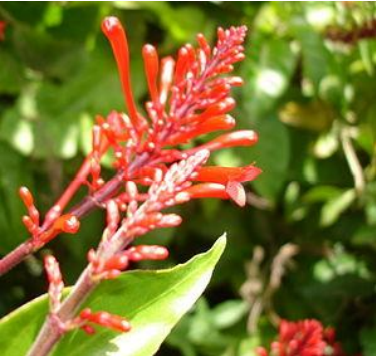
\includegraphics[width=0.8\linewidth]{../../code/tree.png}
   \end{center}
   \caption{Origin picture with some noise.}
   \label{fig:long}
   \label{fig:onecol}
\end{figure}

\begin{figure}[htb]
   \begin{center}
      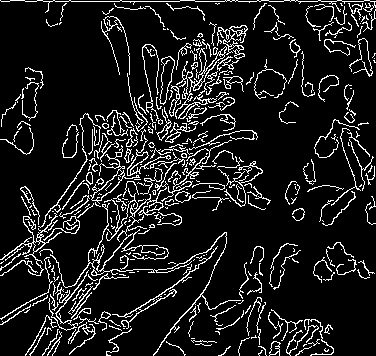
\includegraphics[width=0.8\linewidth]{../../code/cannyTree.png}
   \end{center}
   \caption{Using Canny detector without Guassian smooting.}
   \label{fig:long}
   \label{fig:onecol}
\end{figure}
     
\begin{figure}[htb]
   \begin{center}
      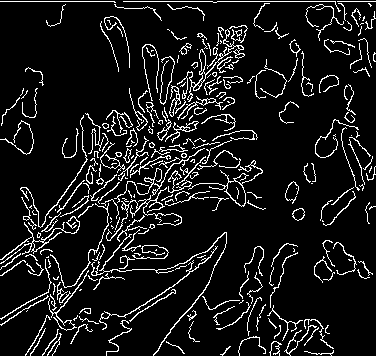
\includegraphics[width=0.8\linewidth]{../../code/cannyTree1.png}
   \end{center}
   \caption{Using Canny detector with Guassian smooting (3 $\times$ 3).}
   \label{fig:long}
   \label{fig:onecol}
\end{figure}

\begin{figure}[htb]  
   \begin{center}
      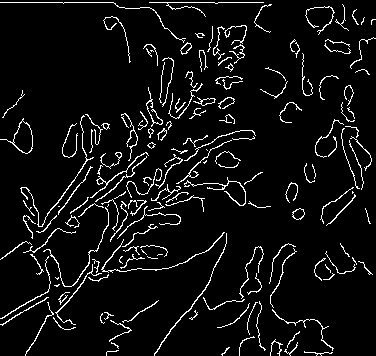
\includegraphics[width=0.8\linewidth]{../../code/cannyTree2.png}
   \end{center}
   \caption{Using Canny detector with Guassian smooting (9 $\times$ 9).}
   \label{fig:long}
   \label{fig:onecol}
\end{figure}

\subsection{Sobel operator}

Sobel operator is a simple edge detector. It is relatively cheap in terms 
of calculations because of using small, sparable integer-valued filter to 
convolving image in the horizontal and vertical directions. But the gradient 
approximation it produces is relatively rough for high-frequency changes in 
the image.

\subsubsection{Formulation}

This operator uses two 3*3 kernel which are convolved with the original 
image to compute the approximations\cite{ref4}. Define $A$ as the source image and 
$G_x$ and $G_y$ are two images that at each point contain the vertical and 
horizontal derivative approximations.

$$
\begin{aligned}
G_x & = 
	\begin{bmatrix}
		+1 & 0 & -1 \\
		+2 & 0 & -1 \\
		+2 & 0 & -2 \\
	\end{bmatrix} * A \\
    & = 
	\begin{bmatrix}
		1 \\ 2 \\ 1
	\end{bmatrix} * (
	\begin{bmatrix}
		+1 & 0 & -1
	\end{bmatrix}	* A) \\
G_y & = 
	\begin{bmatrix}
		+1 & +2 & +1 \\
		0 & 0 & 0 \\
		-1 & -2 & -1 \\
	\end{bmatrix} * A \\
    & = 
	\begin{bmatrix}
		+1 \\ 0 \\ -1
	\end{bmatrix} * (
	\begin{bmatrix}
		1 & 2 & 1
	\end{bmatrix}	* A) \\
\end{aligned}•
$$

Based on the definity of image gradient, the gradient produced by sobel operator 
is 
$$
G = \sqrt{G_x^2 + G_y^2}
$$

And the direction of gradient is 
$$
\Theta = \arctan{\left( \frac{G_y}{G_x} \right)}
$$

The pseudocode implementation is: 

\begin{algorithm}
	\caption{sobel operator}
	\begin{algorithmic}[1]
		\Require $A$: 2D image array
		\Ensure $image$
		\Function {sobel}{$A$}
			\State Gx = [-1 0 1; -2 0 2; -1 0 1] 
			\State Gy = [-1 -2 -1; 0 0 0; 1 2 1]
			\State
			\State rows = size(A, 1)
			\State columns = size(A, 2)
			\State mag = zeros(A)
			\State
			\For{each $i \in [1, rows - 2]$}
				\For{each $j \in [1, columns - 2$}
					\State S1 = sum(sum(Gx .* A (i:i+2, j:j+2)))
					\State S2 = sum(sum(Gy .* A (i:i+2, j:j+2)))
					\State
					\State mag(i + 1, j + 1) = sqrt(S1 .\^{} 2 + S2 .\^{} 2)
				\EndFor
			\EndFor
			\State
			\State threshold = 70 \% $threshold \in [0, 255]$
			\State outputImage = max(mag, threshold)
			\State outputImage(outputImage == round(threshold)) = 0
			\State
			\State \Return outputImage
		\EndFunction
	\end{algorithmic}
\end{algorithm}

\subsubsection{Extension to other demision}

Sobel operator can be divided into 2 operations\cite{ref5}: 

\begin{itemize}[noitemsep]
\item Smoothing perpendicular to the derivative direction with a filter: 
$h(-1) = 1, h(0) = 2, h(1) = 1$
\item Simple central difference in the derivative direction: 
$h'(-1) = 1, h'(0) = 0, h'(1) = -1$
\end{itemize}

From 3D to 4D, suppose that $x, y, z, t \in \{-1, 0, 1\}$: 

3D: 
$$
\begin{aligned}
h'_x(x, y, z) & = h'(x)h(y)h(z) \\
h'_y(x, y, z) & = h(x)h'(y)h(z) \\
h'_z(x, y, z) & = h(x)h(y)h'(z) \\
\end{aligned}
$$

4D: 
$$
\begin{aligned}
h'_x(x, y, z) & = h'(x)h(y)h(z)h(t) \\
h'_y(x, y, z) & = h(x)h'(y)h(z)h(t) \\
h'_z(x, y, z) & = h(x)h(y)h'(z)h(t) \\
h'_t(x, y, z) & = h(x)h(y)h(z)h'(t) \\
\end{aligned}
$$

An example in z-direction in 3D  space: 

$$
\begin{aligned}
h'_z(:, :, -1) & = 
	\begin{bmatrix}
		+1 & +2 & +1 \\
		+2 & +4 & +2 \\
		+1 & +2 & +1 \\
	\end{bmatrix} \\
h'_z(:, :, 0) & = 
	\begin{bmatrix}
		0 & 0 & 0 \\
		0 & 0 & 0 \\
		0 & 0 & 0 \\
	\end{bmatrix} \\
h'_z(:, :, 1) & =
	\begin{bmatrix}
		-1 & -2 & -1 \\
		-2 & -4 & -2 \\
		-1 & -2 & -1 \\
	\end{bmatrix} \\
\end{aligned}
$$

\subsubsection{Optimized operators}

Using central differences, sobel operator does not have perfect rotational symmetry. 
So Scharr try to improve this operator.\cite{ref6,ref7} This is the most frequently used: 

$$
\begin{aligned}
G_x & = 
	\begin{bmatrix}
		+3 & 0 & -3 \\
		+10 & 0 & -10 \\
		+3 & 0 & -3 \\
	\end{bmatrix} \\
G_y & = 
	\begin{bmatrix}
		+3 & +10 & +3 \\
		0 & 0 & 0 \\
		-3 & -10 & -3 \\
	\end{bmatrix}•
\end{aligned}
$$

Kayyali operator was generated from Sobel operator, which is a perfect rotational 
symmetry based convolution filter $3 \times 3$.\cite{ref8} 

Kroon designed a differential filter by using the numerical method optimization.\cite{ref9} 
Kroon use a quasi Newton optimizer from called FMINLBFGS. And he found the radio 
between the kernel values $p_1$ and $p_2$ is 3.5887, which is close to the radio 
of Scharrs kernel $3 \frac{1}{3}$. The operator is: 

$$
\begin{bmatrix}
		+17 & 0 & -17 \\
		+61 & 0 & -61 \\
		+17 & 0 & -17\\
\end{bmatrix}
\qquad
\begin{bmatrix}
	+17 & +61 & +17 \\
	0 & 0 & 0 \\
	-17 & -61 & -17\\
\end{bmatrix}
$$

These matrice are equal to that of a truncated Gaussian derivative of $\sigma = 0.548$, 
which toprevent large aliasing errors with area sampling of the kernel. 

Instead of using a $3 \times 3$ derivative kernel, using a $5 \times 5$ kernel can 
optimized parameter $\sigma$ to $\sigma = 0.6769$ and give the minimal angle erroris:

$$
\begin{aligned}
& \begin{bmatrix}
	0.0007 & 0.0053 & 0 & -0.0053 & -0.0007 \\
	0.0108 & 0.0863 & 0 & -0.0863 & -0.0108 \\
	0.0270 & 0.2150 & 0 & -0.2150 & -0.0270 \\
	0.0108 & 0.0863 & 0 & -0.0863 & -0.0053 \\
	0.0007 & 0.0053 & 0 & -0.0108 & -0.0007 \\
\end{bmatrix} \\ \\
& \begin{bmatrix}
	0.0007 & 0.0108 & 0.0270 & 0.0108 & 0.0007 \\
	0.0053 & 0.0863 & 0.2150 & 0.0863 & 0.0053 \\
	0 & 0 & 0 & 0 & 0 \\
	-0.0053 & -0.0863 & -0.2150 & -0.0863 & -0.0053 \\
	-0.0007 & -0.0108 & -0.0270 & -0.0108 & -0.0007 \\
\end{bmatrix} \\
\end{aligned}
$$

Figure 5-6 show examples processed with the Sobel operator and the Scharr operator.

\begin{figure}[htp]
	\begin{center}
		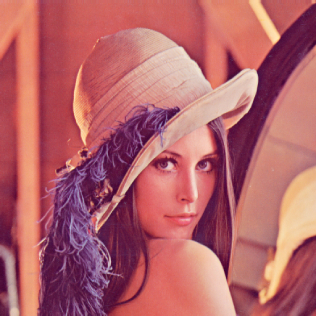
\includegraphics[width=.473\linewidth]{../../code/Lenna.jpg} \quad
		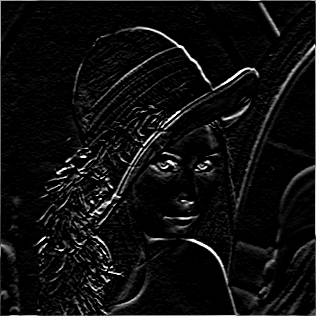
\includegraphics[width=.473\linewidth]{../../code/lenaSobelX.png} \\ 
		\caption{Origin picture without any process. }
		\caption{Origin picture processed by Sobel detector at X direction. }
		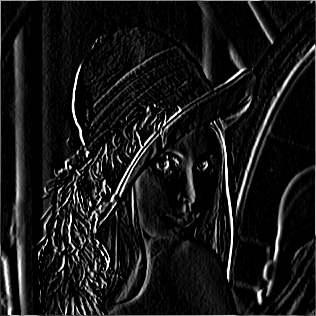
\includegraphics[width=.473\linewidth]{../../code/lenaSobelY.png} \quad
		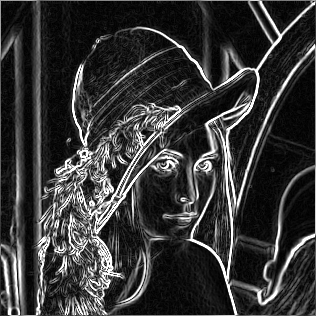
\includegraphics[width=.473\linewidth]{../../code/lenaSobel.png}	
		\caption{Origin picture processed by Sobel detector at Y direction. }
		\caption{Origin picture processed by Sobel detector at X and Y direction. }
		\label{fig:long}
	\end{center}
\end{figure}

\begin{figure}[htp]
	\begin{center}
		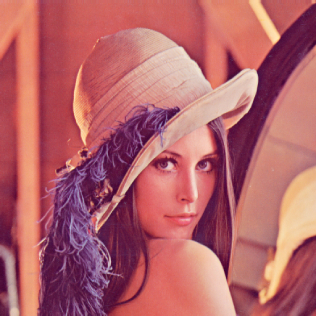
\includegraphics[width=.473\linewidth]{../../code/Lenna.jpg} \quad
		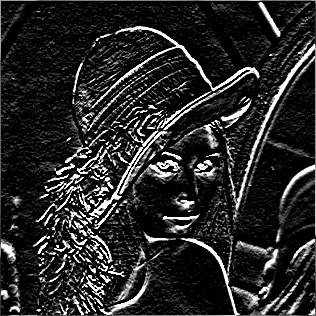
\includegraphics[width=.473\linewidth]{../../code/lenaScharrX.png} \\ 
		\caption{Origin picture without any process. }
		\caption{Origin picture processed by Scharr detector at X direction. }
		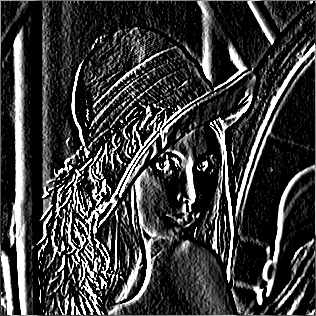
\includegraphics[width=.473\linewidth]{../../code/lenaScharrY.png} \quad
		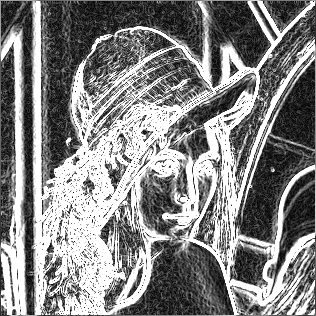
\includegraphics[width=.473\linewidth]{../../code/lenaScharr.png}	
		\caption{Origin picture processed by Scharr detector at Y direction. }
		\caption{Origin picture processed by Scharr detector at X and Y direction. }
		\label{fig:long}
	\end{center}
\end{figure}

\subsection{Canny operator}

Canny edge operator is a widely used edge detection method, which uses the a 
technique that finds the function which optimizes a given functional - calculus 
of variations.\cite{ref10} Compared with Sobel operator, Canny edge detector can better meet 
the following requirements in edge detection: 
\begin{itemize}[noitemsep]
\item Low error rate in edge detection (catch as many edges as possible accurately). 
\item The edge point which detected can be located on the center of the edge accurately. 
\item Ignore or reduce image noise as much as possible in edge detection to preventing 
create error edge. 
\end{itemize}

There are 5 steps in Canny edge detection. 
\begin{enumerate}[noitemsep]
\item Noise reduction. Usually the Gaussian filter is chose to finish it.
\item Get the intensiy gradient of the image. 
\item Using non-maximum supression to get rid of spurious response. 
\item Using double threshold to determin potential edges. 
\item Edge tracking by hysteresis. 
\end{enumerate}

\subsubsection{Noise reduction}

In image detection, image noise can easily affects the result as we talked above. 
So a smoothing filter is needed in deed image pre-processing usually, and Gaussian filter 
is a good choise in most scenarios. The Gaussian filter kernel is convolved with the image can 
sightly reduce the effects of obvious image noise. The equation (size = $(2k + 1) \times (2k + 1)$ 
and suppose that $1 \le i, j \le (2k + 1)$) is: 

$$
\begin{aligned}
H_{ij} & = \frac{1}{2 \pi \sigma^2} \exp{\left( - \frac{[i \ (k + 1)]^2 + [j \ (k + 1)]^2}{2 \sigma^2} \right)}
\end{aligned}
$$

And a $5 \times 5$ size Guassian filter is better for most cases (but we most 
use $3 \times 3$ because it is easily) although it also vary depending on specific 
situations. The is the example: 
$$
B = \frac{1}{159}
	\begin{bmatrix}
		1 & 4 & 5 & 4 & 2 \\
		2 & 9 & 12 & 9 & 4 \\
		5 & 12 & 15 & 12 & 5 \\
		2 & 9 & 12 & 9 & 4 \\
		1 & 4 & 5 & 4 & 2 \\
	\end{bmatrix} \times A
$$

\subsubsection{Get the intensity gradient}

Canny algorithm needs filter to detect horizontal, vertical and diagonal edges (There are 
much more style of edges in real scenes) because an edge may has a variety of directions. 
So using edge detection operator such as Sobel operator or Scharr operator can get the 
value for first derivative in horizontal (suppose $G_x = \frac{\partial f}{\partial x}$
) and vertical (suppose $G_y =  \frac{\partial f}{\partial x}$) direction. The 
gradient and direction are:

$$
\begin{aligned}
& G = \sqrt{G_x^2 + G_y^2} \\
& \Theta = \arctan{\left( \frac{G_y}{G_x} \right)}
\end{aligned}
$$

\subsubsection{Non-maximum suppression}

Non-maximum suppression is applied to find the edge point which have the sharpest 
change in locale area. Operations will be done in each pixel in the image: 
\begin{enumerate}[noitemsep]
\item Compare the edge intensity of the current pixel with the edge intensity of 
the pixel in the positive and negative gradient directions. 
\item Preserve the value if the edge intensity of the current pixel is the largest 
in the mask compared to another pixels with the same direction. Otherwise, suppressed 
the value. 
\end{enumerate}

Suppose that $x'$ and $x''$ are the neighbors of pixel $x$ along normal direction 
to an edge.\cite{ref13} And $|\nabla G|(x, y)$ is the gradient at pixel $(x, y)$, 
Non-maximum suppression can be written as: 
$$
M(x, y) + 
	\begin{cases}
		|\nabla G|(x, y)&, |\nabla G|(x, y) > |\nabla G|(x', y') \\
		& \& |\nabla G|(x, y) > |\nabla G|(x'', y'') \\
		0&, otherwise \\
	\end{cases}
$$

The pseudo code is 
\begin{algorithm}
	\caption{Non-maximum suppression}
	\begin{algorithmic}[1]
		\Require G: the gradient at each pixel in the image
		\Require $(x', y')$, $(x'', y'')$: the neighbors of pixel $(x, y)$
		\Ensure $I_N$: result image
		\For {each pixel $(x, y)$} 
			\If {$G(x, y) > G(x', y')$ and $G(x, y) > G(x'', y'')$}
			\State {$I_N(x, y) = G(x, y)$} 
			\Else
			\State {$I_N(x, y) = 0$}
			\EndIf
		\EndFor
	\end{algorithmic}
\end{algorithm}

\subsubsection{Double threshold}

A more accurae representation of real edges can be shown by using non-maximum 
suppression. But some pixels may remain which caused by noise or color variation. 
In Sobel operator, we use a threshold to distinguish whether the pixel is in edge 
or not. It can be easliy used but likely ignore some potential edges. 

So Canny use double threshold\cite{ref10}, which can find more potential details 
of edge and also increase the complexity of calculating. Suppose $p_1 < p_2$ are 
2 values of threshold, they divides gradients we get in prvious steps into 3 
intervals. Suppose $G_{xy}$ as the gredient at pixel$(x, y)$, the 3 interval can
be given as: 
$$
\text{point $(x, y)$} = 
	\begin{cases}
		\text{not a edge}, & G_{xy} < p_1 \\
		\text{weak edge}, & p_1 \le G_{xy} < p_2 \\
		\text{strong edge}, & p_2 \le G_{xy} \\
	\end{cases}
$$

The ``weak edge'' need further processing, and it would be done in the next step. 

\subsubsection{Track by hystersis}

Weak edge pixels can either be extracted from the true edge, or the noise/color 
variations. So it is necessary to remove the weak edges that caused by the latter 
reasons to approach a more accurate result. 

Pixel$(x, y)$ in the image has 8 neighbors and is a weak edge. We consider this 
pixel is a true edge if there is at least one neighbor is a strong edge. Otherwise, 
it is not a true edge. It can be written as 
$$
\text{point $(x, y)$} = 
	\begin{cases}
		\text{not a edge}, & \text{none of neighbors} \\
			& \text{was a strong edge} \\
		\text{true edge}, &  \text{at least one neighbors} \\
			& \text{is a string edge} \\
	\end{cases}
$$

\subsubsection{Development}

In original Canny edge detector, non-maximum suppression only apples at 4 angle, 
which are 0°, 45°, 90° and 135° that define 8 direction.\cite{ref10} The 8 directions are: 

\begin{itemize}[noitemsep]
\item The point will be considered to be in the {\bf east and west} directions if the 
rounded gradient angle is 0°. 
\item The point will be considered to be in the {\bf north east and south west} directions if the 
rounded gradient angle is 45°. 
\item The point will be considered to be in the {\bf north and south} directions if the 
rounded gradient angle is 90°. 
\item The point will be considered to be in the {\bf sourth east and north west} directions if the 
rounded gradient angle is 135°. 
\end{itemize}

It is definitly that use this simplified method can get edges in more directions and effective 
in image processing. But someone proposed to use interpolation to imporve Canny detector at 
this step and here are the reasons: 
\begin{enumerate}[label={\alph*)}]
\item Edge gradient directions in the natural image are not necessarily along the 8 directions.
In order to find the gradient direction that best matches its location on a pixel, the 
pixel value on both sides of must be interploated; 
\item Also because that the pixels in the actual digital image are discrete two-dimensional 
matrices, the point on both sides of the gradient directions at the true center position, or 
be called as sub-pixels, do not necessarily exist. The non-existent point and the gradient 
value of this point can only be obtained by interpolating the points on both side of it.
\end{enumerate}

There are 2 set of pictures reflect the result about Canny edge detection and compression 
between non-maximum supression without interpolation and non-maximum suppresion 
with interpolation. 

\begin{figure}[htp]
	\begin{center}
		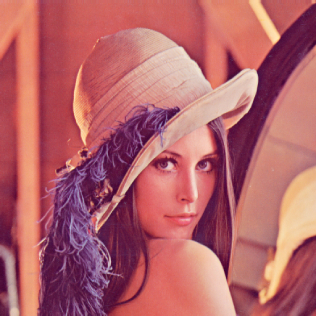
\includegraphics[width=1\linewidth]{../../code/Lenna.jpg} \\ 
		\caption{orgin picture}
		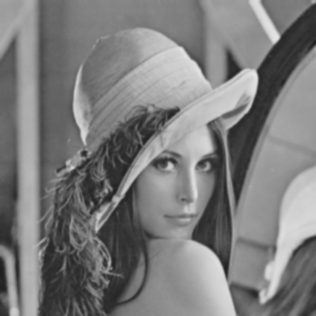
\includegraphics[width=.473\linewidth]{../../code/cannyGuassianLena.png} \quad
		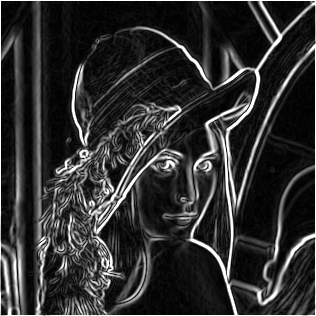
\includegraphics[width=.473\linewidth]{../../code/cannySobelLena.png} \\
		\caption{Step 1: Process with Gaussian filter.}
		\caption{Step 2: Process with Sobel detector.}
		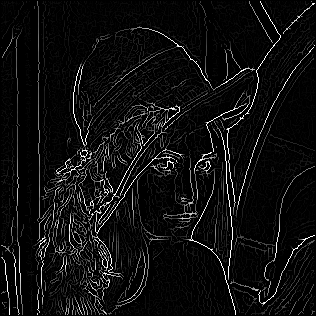
\includegraphics[width=.473\linewidth]{../../code/cannySuppressionPaperLena.png} \quad
		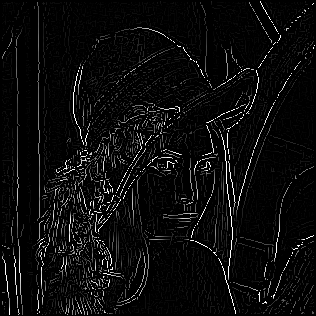
\includegraphics[width=.473\linewidth]{../../code/cannySuppressionInterpolationLena.png} \\
		\caption{Step 3: Non-maximum suppression without interpolation. }
		\caption{Step 3: Non-maximum suppression with interpolation. } 
		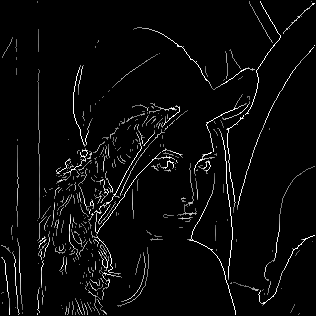
\includegraphics[width=.473\linewidth]{../../code/cannyThresholdPaperLena.png}	\quad
		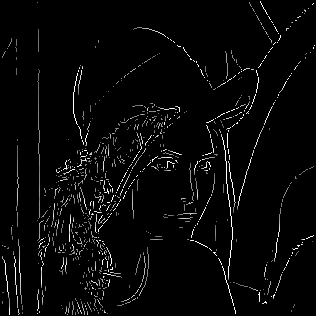
\includegraphics[width=.473\linewidth]{../../code/cannyThresholdInterpolationLena.png} \\
		\caption{Step 4-5: Hysteresisi thresholding without interpolation at step 3. }
		\caption{Step 4-5: Hysteresisi thresholding with interpolation at step 3. }
		\label{fig:long}
	\end{center}
\end{figure}

\begin{figure}[htp]
	\begin{center}
		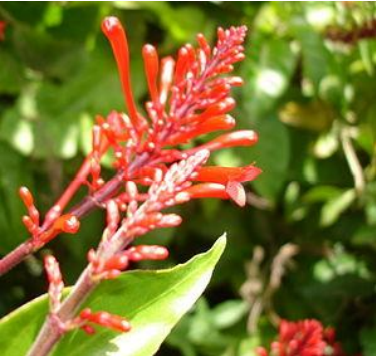
\includegraphics[width=1\linewidth]{../../code/tree.png} \\ 
		\caption{orgin picture}
		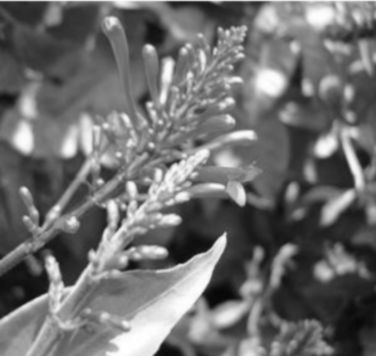
\includegraphics[width=.473\linewidth]{../../code/cannyGuassianTree.png} \quad
		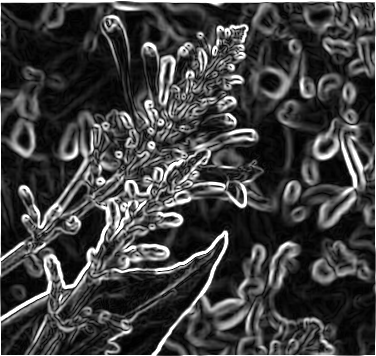
\includegraphics[width=.473\linewidth]{../../code/cannySobelTree.png} \\
		\caption{Step 1: Process with Gaussian filter.}
		\caption{Step 2: Process with Sobel detector.}
		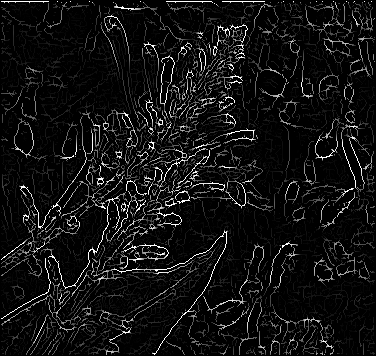
\includegraphics[width=.473\linewidth]{../../code/cannySuppressionPaperTree.png} \quad
		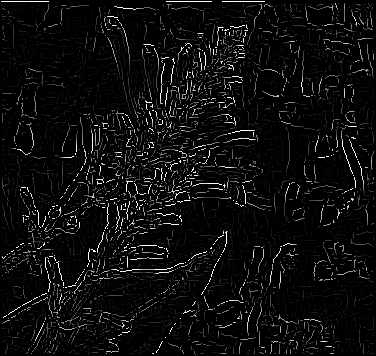
\includegraphics[width=.473\linewidth]{../../code/cannySuppressionInterpolationTree.png} \\
		\caption{Step 3: Non-maximum suppression without interpolation. }
		\caption{Step 3: Non-maximum suppression with interpolation. }
		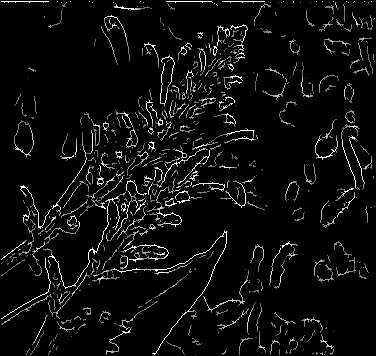
\includegraphics[width=.473\linewidth]{../../code/cannyThresholdPaperTree.png}	\quad
		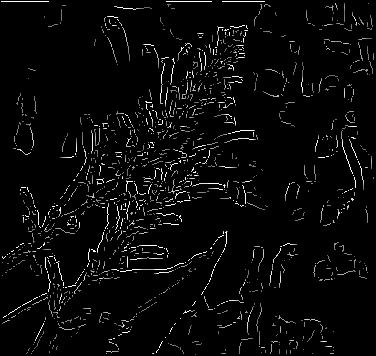
\includegraphics[width=.473\linewidth]{../../code/cannyThresholdInterpolationTree.png} \\
		\caption{Step 4-5: Hysteresisi thresholding without interpolation at step 3. }
		\caption{Step 4-5: Hysteresisi thresholding with interpolation at step 3. }
		\label{fig:long}
	\end{center}
\end{figure}

By comparing the pictures generated at each step, here are some differeces: 
\begin{enumerate}[noitemsep]
\item Edge pixels filtered out by the interpolation method are less than edge 
processed without interpolation, so image processed with interpolation looks not 
very continuous in some place, which also make the loss of image details. 
\item However, non-maximum suppression without interpolation is more likely to 
get an edge with a width greater than 1 pixel in terms of edge width. So in case 
of high-precision single-point response, non-maximum suppression with interpolation 
may have a better result. 
\end{enumerate}

\subsubsection{Deriche edge detector}

Deriche edge detector is a edge detection operetor that based on Canny edge detector 
developed by Rachid Deriche in 1987 (Canny edge detector was published in 1986). 
There are 4 steps in the algorithm, some of which is similar as Canny detector: 
\begin{enumerate}[noitemsep]
\item Smoothing. This step using IIR filter instead of Guassian filter. 
\item Calculation of magnitude and gradient direction
\item Non-maximum suppression
\item Double threshold
\item Hystersis threshold with double thresholds
\end{enumerate}

The difference between Canny edge detector and Deriche edge detector are in step 1 
and step 2. IIR ({\bf I}nfinite {\bf I}mpulse {\bf R}esponse) filter is used to 
replace Gussian filter. Deriche propose 2 filters\cite{ref12} to optimize the Canny 
criteria. 

The first is 
$$
f(x) = \frac{S}{\omega} e^{\alpha |x|} \sin{\omega x}
$$

Through mathematical inference and calculations and experiments\cite{ref12}, Deriche 
obtain the most effective filter when the value of $\omega$ approaches 0.By that 
the second formula can be given as 
$$
f(x) = Sxe^{-\alpha |x|}
$$

Using the filter, Deriche edge detector can be able to process image in a short 
constant time independent of the desired amount of smoothing when the processed 
image is very noisy or requires a lots of smoothing. And these two filters have 
only one parameter so that changing the characteristics of image processed can 
be more easily. 

\section{Conclusion}

By reading relative papers and materials, I understand these edge detectors more 
deeply with learning their priciple, specific steps and running code to precess 
example picture. It is not a easy journey for me, but I was glad to see these 
different pictures that computer shown when my computer run code successfully. 

These edge detectors definitly are not perfect. With the image processed by 
edge detector the loss of amount of data reduce the possibility of human 
identification, but the remaining features can be stored by computer and be used 
to detect objects. 

Whether it is the Sobel, Scharr, Canny and Deriche edge detector, they are 
first-order edge detector and proposed before 1990s, and now there are many kinds 
of methods that be different with these ``traditional'' approaches, which named 
deep-learning based approaches. 

Deep-learning based approaches can be divided into 5 classes. They are general 
edge detection, object contour detection, semantic edge detection(Category-Aware) 
occlusion boundary detection and edge detection from multi-frames.\cite{ref13} 

The world is developing rapidly and I also should learn these cutting-edge 
technologies hard.

%%%%%%%%%% REFERENCE

\begin{thebibliography}{99}
\bibitem{ref1} H.G. Barrow and J.M. Tenenbaum (1981) ``Interpreting line drawings 
as three-dimensional surfaces'', Artificial Intelligence, vol 17, issues 1–3, pages 75–116.
\bibitem{ref2} Lindeberg, Tony (2001) [1994],``Edge detection'', Encyclopedia of 
Mathematics, EMS Press.
\bibitem{ref3} Irwin Sobel, 2014, History and Definition of the Sobel Operator.
\bibitem{ref4} K. Engel (2006). Real-time volume graphics. pp.
\bibitem{ref5} Scharr, Hanno, 2000, Dissertation (in German), Optimal Operators 
in Digital Image Processing. 
\bibitem{ref6} B. Jähne, H. Scharr, and S. Körkel. Principles of filter design. 
In Handbook of Computer Vision and Applications. Academic Press, 1999.
\bibitem{ref7} Dim, Jules R.; Takamura, Tamio (2013-12-11). "Alternative Approach 
for Satellite Cloud Classification: Edge Gradient Application". Advances in Meteorology. 
2013: 1–8. doi:10.1155/2013/584816. ISSN 1687-9309.
\bibitem{ref8} D. Kroon, 2009, Short Paper University Twente, Numerical Optimization 
of Kernel Based Image Derivatives.
\bibitem{ref9} J. Canny, "A Computational Approach to Edge Detection," in IEEE 
Transactions on Pattern Analysis and Machine Intelligence, vol. PAMI-8, no. 6, pp. 679-698, 
Nov. 1986, doi: 10.1109/TPAMI.1986.4767851.
\bibitem{ref10} A. Neubeck and L. Van Gool, "Efficient Non-Maximum Suppression," 
18th International Conference on Pattern Recognition (ICPR'06), Hong Kong, 2006, 
pp. 850-855, doi: 10.1109/ICPR.2006.479.
\bibitem{ref11} R. Deriche, Using Canny's criteria to derive a recursively 
implemented optimal edge detector, Int. J. Computer Vision, Vol. 1, pp. 167–187, April 1987.
\bibitem{ref12} Alper Yilmaz, Mubarak Shah Fall 2012, UCF
\bibitem{ref13} MarkMoHR, Awesome-Edge-Detection-Papers(
\url{https://github.com/MarkMoHR/Awesome-Edge-Detection-Papers}), github
\end{thebibliography}

%{\small
%\bibliographystyle{ieee_fullname}
%\bibliography{egbib}
%}

\end{document}
